\documentclass[11pt,a4paper]{article}

% Packages
\usepackage[utf8]{inputenc}
\usepackage[margin=1in]{geometry}
\usepackage{amsmath,amssymb,amsthm}
\usepackage{graphicx}
\usepackage{tikz}
\usetikzlibrary{arrows.meta,positioning,calc}
\usepackage{hyperref}
\usepackage{cleveref}
\usepackage{caption}
\usepackage{subcaption}

% Title and author
\title{\textbf{The Equivalent Couple Problem in Inverse Dynamics Analysis of Closed-Loop Systems}}
\author{Dieter}
\date{\today}

% Custom commands
\newcommand{\bvec}[1]{\mathbf{#1}}
\newcommand{\Feq}{\bvec{F}_{\text{eq}}}
\newcommand{\Ceq}{C_{\text{eq}}}

\begin{document}

\maketitle

\begin{abstract}
Inverse dynamics analysis provides a powerful tool for understanding forces and moments in biomechanical systems such as the golf swing. However, the interpretation of results requires careful consideration of the mathematical framework underlying the method. This article examines a fundamental limitation of inverse dynamics when applied to closed-loop systems: the ambiguity inherent in the ``equivalent couple'' representation. We demonstrate that a force and couple calculated at one point on a rigid body (typically the midpoint of the hands on a golf club) may correspond to multiple physically distinct force distributions applied by the golfer. Through mathematical analysis and concrete examples, we show how the point of force application significantly affects the interpretation of inverse dynamics results, with implications for understanding skilled motor control and the ongoing debate about torque application in golf.
\end{abstract}

\section{Introduction}

Inverse dynamics (also called reverse dynamics) is a computational technique that calculates the forces and moments required to produce an observed motion. In golf biomechanics, this method takes motion capture data of a club and golfer and computes the equivalent forces and couples acting at a reference point—typically the midpoint between the hands on the grip.

The appeal of inverse dynamics lies in its apparent simplicity: it reduces the complex multi-point force application from fingers, palms, and thumbs to a single force vector and a single couple (torque) at a reference point. However, this mathematical convenience masks a critical interpretive challenge: \emph{the same force-couple pair at one point can arise from infinitely many different force distributions applied to the club}.

This article explores the mathematical basis for this ambiguity and its practical implications. We show that:
\begin{itemize}
    \item A couple measured at the grip midpoint does not necessarily indicate a twisting action by the golfer
    \item The location where forces are applied (e.g., fingers vs. palm, left hand vs. right hand) fundamentally changes the equivalent couple
    \item Without additional information about force distribution, inverse dynamics results have inherent interpretive limits
\end{itemize}

\section{Mathematical Background: Force-Couple Equivalence}

\subsection{The Fundamental Principle}

In rigid body mechanics, any system of forces can be reduced to a statically equivalent system consisting of a single resultant force and a couple acting at an arbitrary reference point. This equivalence is \emph{dynamic}—both systems produce identical linear and angular accelerations of the rigid body.

Consider a force $\bvec{F}$ applied at a point displaced by distance $\bvec{d}$ from a reference point. This force can be equivalently represented at the reference point as:
\begin{itemize}
    \item The same force $\bvec{F}$ (translational effect)
    \item A couple $\bvec{C} = \bvec{d} \times \bvec{F}$ (rotational effect)
\end{itemize}

The key insight is that \emph{the couple is a free vector}—it can act anywhere on the rigid body without changing the body's motion. The force, however, is bound to its line of action; moving the point of application requires introducing or modifying the couple to maintain equivalence.

\subsection{Transforming Between Reference Points}

If inverse dynamics yields a force $\Feq$ and couple $\Ceq$ at reference point $m$ (midpoint), we can transform these to an equivalent force and couple at any other point along the grip. 

For a one-dimensional analysis along the grip axis (labeled by positions $t$, $m$, $b$ for top, middle, bottom), the relationship is:

\begin{equation}
\label{eq:couple_transform}
C_i = M_m \left(1 - \frac{d_i}{d_m}\right) + C_m
\end{equation}

where:
\begin{itemize}
    \item $C_i$ is the equivalent couple at point $i$
    \item $M_m$ is the moment of force about the midpoint
    \item $d_i$ is the distance from the center of mass to point $i$
    \item $d_m$ is the distance from the center of mass to midpoint $m$
    \item $C_m$ is the couple at the midpoint from inverse dynamics
\end{itemize}

\begin{figure}[ht]
\centering
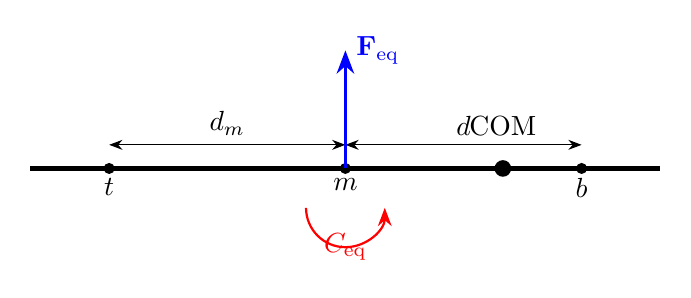
\begin{tikzpicture}[>=Stealth]
    % Draw club shaft
    \draw[line width=2pt] (0,0) -- (8,0);
    
    % Mark points
    \fill (1,0) circle (2pt) node[below] {$t$};
    \fill (4,0) circle (2pt) node[below] {$m$};
    \fill (7,0) circle (2pt) node[below] {$b$};
    
    % Draw distance markers
    \draw[<->] (1,0.3) -- (4,0.3) node[midway,above] {$d_m$};
    \draw[<->] (4,0.3) -- (7,0.3) node[midway,above] {$d$};
    
    % Draw COM
    \fill (6,0) circle (3pt) node[above=3mm] {COM};
    
    % Draw force at midpoint
    \draw[->,very thick,blue] (4,0) -- (4,1.5) node[right] {$\Feq$};
    
    % Draw couple symbol at midpoint
    \draw[->,red,thick] (3.5,-0.5) arc (180:360:0.5);
    \node[red] at (4,-1) {$\Ceq$};
\end{tikzpicture}
\caption{Schematic of golf club grip showing reference points (top, middle, bottom) and center of mass (COM). Inverse dynamics typically reports an equivalent force $\Feq$ and couple $\Ceq$ at the midpoint $m$.}
\label{fig:grip_schematic}
\end{figure}

\subsection{The Range of Possible Couples}

From Equation~\ref{eq:couple_transform}, we can determine the range of possible equivalent couples for a given inverse dynamics result. At the top of the grip ($t$):

\begin{equation}
C_t = M_m \left(1 - \frac{d_t}{d_m}\right) + C_m
\end{equation}

At the bottom of the grip ($b$):

\begin{equation}
C_b = M_m \left(1 - \frac{d_b}{d_m}\right) + C_m
\end{equation}

The range of viable equivalent couples spans from $C_b$ to $C_t$. Critically, \emph{this range increases with the moment of force} $M_m = F \cdot d_m$. For larger forces or forces applied farther from the center of mass, the uncertainty in the ``true'' couple grows substantially.

\section{Physical Interpretation: What Does a Couple Really Mean?}

\subsection{The Misconception}

A common interpretation of inverse dynamics results is:
\begin{quote}
    ``If inverse dynamics shows a force of $F$ and a couple of $C$ at the grip midpoint, then the golfer must be applying a linear push/pull of magnitude $F$ and simultaneously twisting with torque $C$.''
\end{quote}

This interpretation is \textbf{not generally valid}. Here's why:

\subsection{The Reality: Distributed Forces}

Golfers do not apply forces at a single point or apply pure couples. Instead, they apply forces at multiple locations on the grip:
\begin{itemize}
    \item Pressure from the pads of fingers
    \item Pushing with the heel of the palm
    \item Pulling with specific fingers (e.g., pinky of left hand)
    \item Directional forces from thumbs
\end{itemize}

Each of these distributed forces contributes to both the net force and the equivalent couple measured at the midpoint. Importantly, \emph{a couple can arise purely from offset forces, without any actual twisting action}.

\begin{figure}[ht]
\centering
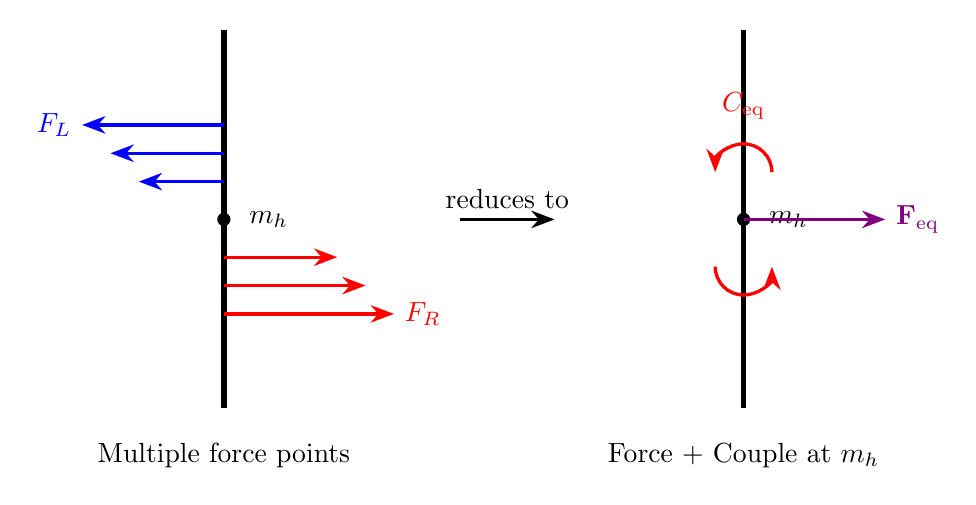
\begin{tikzpicture}[>=Stealth,scale=1.2]
    % Left diagram - forces above and below midpoint
    \begin{scope}
        \draw[line width=2pt] (0,0) -- (0,4);
        \fill (0,2) circle (2pt) node[right=2mm] {$m_h$};
        
        % Multiple forces
        \draw[->,very thick,blue] (0,3) -- (-1.5,3) node[left] {$F_L$};
        \draw[->,very thick,blue] (0,2.7) -- (-1.2,2.7);
        \draw[->,very thick,blue] (0,2.4) -- (-0.9,2.4);
        
        \draw[->,very thick,red] (0,1.6) -- (1.2,1.6);
        \draw[->,very thick,red] (0,1.3) -- (1.5,1.3);
        \draw[->,very thick,red] (0,1) -- (1.8,1) node[right] {$F_R$};
        
        \node at (0,-0.5) {Multiple force points};
    \end{scope}
    
    % Arrow
    \draw[->,very thick] (2.5,2) -- (3.5,2) node[midway,above] {reduces to};
    
    % Right diagram - equivalent at midpoint  
    \begin{scope}[shift={(5.5,0)}]
        \draw[line width=2pt] (0,0) -- (0,4);
        \fill (0,2) circle (2pt) node[right=2mm] {$m_h$};
        
        % Net force
        \draw[->,very thick,violet] (0,2) -- (1.5,2) node[right] {$\Feq$};
        
        % Couple
        \draw[->,red,very thick] (-0.3,1.5) arc (180:360:0.3);
        \draw[->,red,very thick] (0.3,2.5) arc (0:180:0.3);
        \node[red] at (0,3.2) {$\Ceq$};
        
        \node at (0,-0.5) {Force + Couple at $m_h$};
    \end{scope}
\end{tikzpicture}
\caption{Distributed forces from multiple contact points (left) reduce to an equivalent single force and couple at the midpoint (right). The couple arises from the spatial distribution of forces, not necessarily from a twisting action.}
\label{fig:force_reduction}
\end{figure}

\subsection{A Thought Experiment: Single Force Off-Center}

Consider a hypothetical scenario where a golfer applies force at only one point on the grip, but that point is not at the midpoint. Let's say a force $F$ is applied at distance $d_F$ from the midpoint.

\textbf{Forward dynamics view:} This is just a single force—no couple exists in reality.

\textbf{Inverse dynamics result at midpoint:}
\begin{itemize}
    \item Net force: $F$
    \item Equivalent couple: $C = F \cdot d_F$
\end{itemize}

The inverse dynamics analysis \emph{creates} a couple to account for the offset, even though no twisting action occurs. This demonstrates that the presence of a couple in inverse dynamics results does not prove the golfer is twisting the club.

\section{Quantitative Analysis: The Ambiguity Problem}

\subsection{Case Study: Top of Backswing}

Let's examine a specific scenario at the top of the backswing. Suppose inverse dynamics yields:
\begin{itemize}
    \item Positive moment of force about the midpoint (force acts upward, creating clockwise rotation tendency)
    \item Positive couple (clockwise twisting at midpoint)
\end{itemize}

Now consider two different force application patterns that could produce these results:

\textbf{Case A:} Primary force applied at the right forefinger (higher than midpoint)

\textbf{Case B:} Primary force applied at the left thumb (closer to midpoint)

Using Equation~\ref{eq:couple_transform}, the equivalent couple at the actual point of force application differs between these cases:

\begin{align}
C_A &= M_m \left(1 - \frac{d_A}{d_m}\right) + C_m \\
C_B &= M_m \left(1 - \frac{d_B}{d_m}\right) + C_m
\end{align}

Since $d_A > d_B$ (forefinger is farther from COM than thumb), we have:
\begin{equation}
C_A < C_B
\end{equation}

In Case A, the equivalent couple at the right forefinger is \emph{lower} than the couple reported at the midpoint, even though the inverse dynamics gives the same force-couple pair at the midpoint for both cases.

\begin{figure}[ht]
\centering
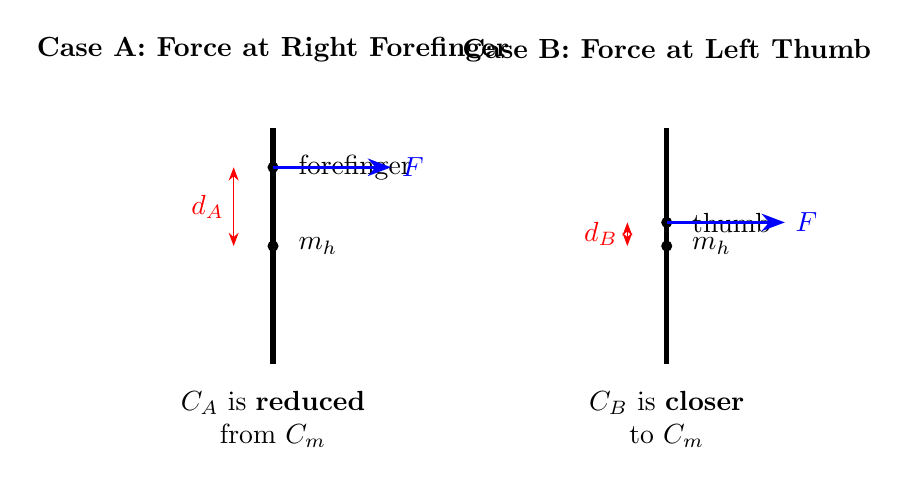
\begin{tikzpicture}[>=Stealth,scale=1.0]
    % Case A
    \begin{scope}
        \node at (0,4) {\textbf{Case A: Force at Right Forefinger}};
        
        % Club
        \draw[line width=2pt] (0,0) -- (0,3);
        \fill (0,1.5) circle (2pt) node[right=2mm] {$m_h$};
        \fill (0,2.5) circle (2pt) node[right=2mm] {forefinger};
        
        % Force
        \draw[->,very thick,blue] (0,2.5) -- (1.5,2.5) node[right] {$F$};
        
        % Distance markers
        \draw[<->,red] (-0.5,1.5) -- (-0.5,2.5) node[midway,left] {$d_A$};
        
        \node[align=center] at (0,-0.7) {$C_A$ is \textbf{reduced}\\from $C_m$};
    \end{scope}
    
    % Case B
    \begin{scope}[shift={(5,0)}]
        \node at (0,4) {\textbf{Case B: Force at Left Thumb}};
        
        % Club
        \draw[line width=2pt] (0,0) -- (0,3);
        \fill (0,1.5) circle (2pt) node[right=2mm] {$m_h$};
        \fill (0,1.8) circle (2pt) node[right=2mm] {thumb};
        
        % Force  
        \draw[->,very thick,blue] (0,1.8) -- (1.5,1.8) node[right] {$F$};
        
        % Distance markers
        \draw[<->,red] (-0.5,1.5) -- (-0.5,1.8) node[midway,left] {$d_B$};
        
        \node[align=center] at (0,-0.7) {$C_B$ is \textbf{closer}\\to $C_m$};
    \end{scope}
\end{tikzpicture}
\caption{Two force application scenarios yielding identical inverse dynamics results at the midpoint but different equivalent couples at the actual point of application.}
\label{fig:case_comparison}
\end{figure}

\subsection{Numerical Example}

Consider concrete numbers based on typical golf swing parameters. Assume:
\begin{itemize}
    \item Grip length from midpoint to club COM: $d_m = 30$ inches
    \item Applied force: $F = 5$ lbs
    \item Moment of force at midpoint: $M_m = 150$ in-lbs
    \item Couple at midpoint from inverse dynamics: $C_m = -35$ in-lbs
\end{itemize}

\textbf{Case A:} Force at right forefinger ($d_A = 32$ inches from COM)
\begin{align}
C_A &= 150 \left(1 - \frac{32}{30}\right) + (-35) \\
    &= 150(-0.0667) - 35 \\
    &= -10 - 35 \\
    &= -45 \text{ in-lbs}
\end{align}

\textbf{Case B:} Force at left thumb ($d_B = 28$ inches from COM)  
\begin{align}
C_B &= 150 \left(1 - \frac{28}{30}\right) + (-35) \\
    &= 150(0.0667) - 35 \\
    &= 10 - 35 \\
    &= -25 \text{ in-lbs}
\end{align}

The equivalent couple differs by 20 in-lbs (about 44\%) depending solely on where the force is applied, despite identical inverse dynamics results.

\subsection{Sign Changes and the Alpha Debate}

In some scenarios, the magnitude of $M_m$ and the distance ratios can be such that the equivalent couple actually \emph{changes sign} when transformed to the actual point of force application.

For late downswing, suppose inverse dynamics gives:
\begin{itemize}
    \item Positive moment of force: $M_m > 0$  
    \item Negative couple: $C_m < 0$
\end{itemize}

At point $i$ where force is primarily applied:
\begin{equation}
C_i = M_m \left(1 - \frac{d_i}{d_m}\right) + C_m
\end{equation}

If $\frac{d_i}{d_m} > 1$ (force applied beyond midpoint toward clubhead) and the ratio satisfies:
\begin{equation}
M_m \left(\frac{d_i}{d_m} - 1\right) > |C_m|
\end{equation}

Then $C_i > 0$, despite $C_m < 0$.

This has direct relevance to the ``alpha torque'' debate in golf biomechanics. Researchers debate whether golfers apply a torque in the direction of rotation (positive alpha) or against it (negative alpha) during the downswing. Our analysis shows that depending on where forces are applied along the grip, the \emph{same inverse dynamics data} could be interpreted as either positive or negative torque at the actual site of force application.

\begin{figure}[ht]
\centering
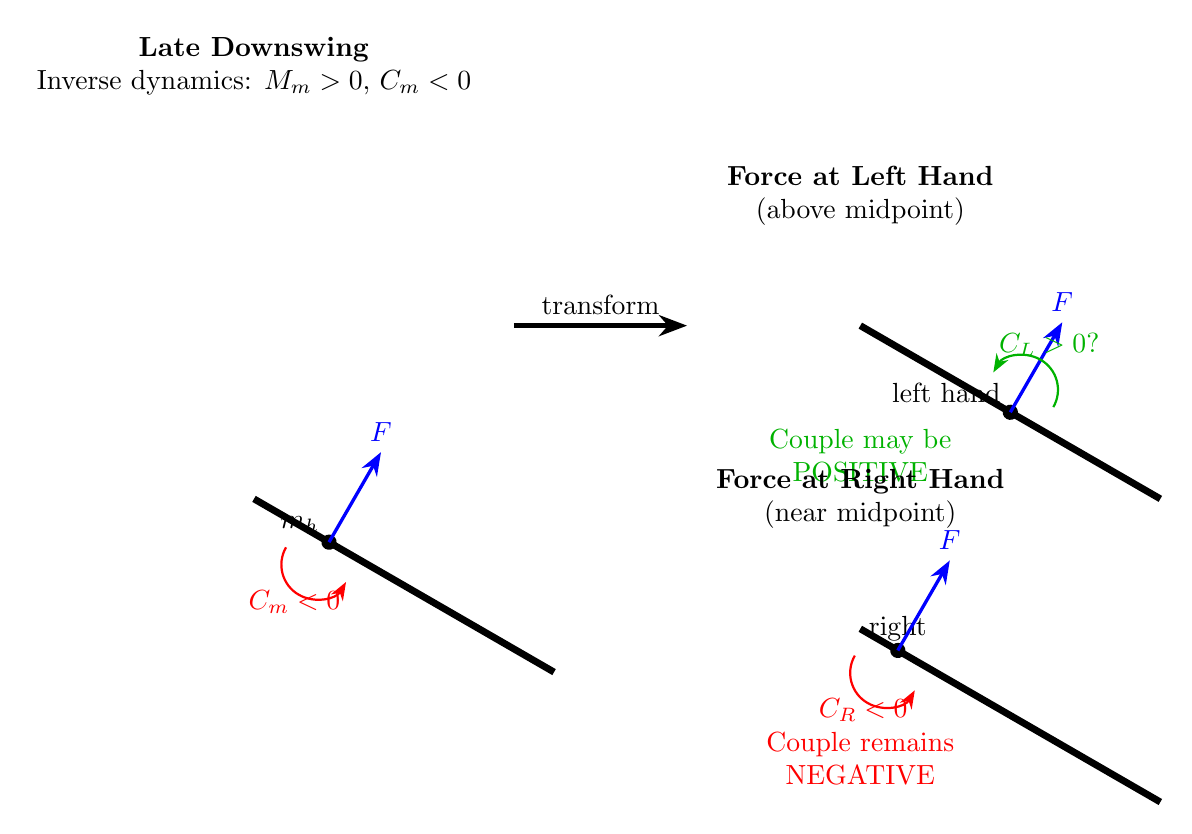
\begin{tikzpicture}[>=Stealth,scale=1.1]
    % Late downswing scenario
    \node[align=center] at (0,5) {\textbf{Late Downswing}\\Inverse dynamics: $M_m > 0$, $C_m < 0$};
    
    % Club in downswing position
    \begin{scope}[rotate=-30]
        \draw[line width=2.5pt] (0,0) -- (4,0);
        \fill (1,0) circle (2.5pt) node[above left] {$m_h$};
        \draw[->,very thick,blue] (1,0) -- (1,1.2) node[above] {$F$};
        
        % Negative couple at midpoint
        \draw[->,red,thick] (0.6,-0.3) arc (180:360:0.4);
        \node[red] at (1,-0.8) {$C_m < 0$};
    \end{scope}
    
    % Transform to actual application point
    \draw[->,ultra thick] (3,2) -- (5,2) node[midway,above] {transform};
    
    % Left hand (higher up grip)
    \begin{scope}[shift={(7,2)}]
        \node[align=center] at (0,1.5) {\textbf{Force at Left Hand}\\(above midpoint)};
        \begin{scope}[rotate=-30]
            \draw[line width=2.5pt] (0,0) -- (4,0);
            \fill (2,0) circle (2.5pt) node[above left] {left hand};
            \draw[->,very thick,blue] (2,0) -- (2,1.2) node[above] {$F$};
            
            % Potentially positive couple
            \draw[->,green!70!black,thick] (2.4,0.3) arc (0:180:0.4);
            \node[green!70!black] at (2,0.9) {$C_L > 0$?};
        \end{scope}
        \node[align=center,green!70!black] at (0,-1.5) {Couple may be\\POSITIVE};
    \end{scope}
    
    % Right hand (lower on grip)
    \begin{scope}[shift={(7,-1.5)}]
        \node[align=center] at (0,1.5) {\textbf{Force at Right Hand}\\(near midpoint)};
        \begin{scope}[rotate=-30]
            \draw[line width=2.5pt] (0,0) -- (4,0);
            \fill (0.5,0) circle (2.5pt) node[above] {right};
            \draw[->,very thick,blue] (0.5,0) -- (0.5,1.2) node[above] {$F$};
            
            % Still negative couple
            \draw[->,red,thick] (0.1,-0.3) arc (180:360:0.4);
            \node[red] at (0.5,-0.8) {$C_R < 0$};
        \end{scope}
        \node[align=center,red] at (0,-1.5) {Couple remains\\NEGATIVE};
    \end{scope}
\end{tikzpicture}
\caption{Late downswing scenario showing how the same inverse dynamics result ($M_m > 0$, $C_m < 0$) can lead to opposite-sign couples depending on force application location. This ambiguity is central to the alpha torque debate.}
\label{fig:alpha_debate}
\end{figure}

\section{Forward Dynamics Perspective: Finding the Meaningful Reference Point}

The analysis so far has shown the problem: inverse dynamics gives one answer, but that answer corresponds to many possible physical realities. Is there a principled way to select the ``right'' reference point for interpretation?

\subsection{The Forward Dynamics Decomposition}

We propose a forward dynamics approach to identify the most physically meaningful reference point:

\textbf{Step 1:} Recognize that multiple forces act on the grip at various locations

\textbf{Step 2:} Resolve these distributed forces into two equivalent forces acting on opposite sides of the shaft
\begin{itemize}
    \item Sum all forces on the left side of the grip → $\bvec{F}_L$ at effective point $L$
    \item Sum all forces on the right side of the grip → $\bvec{F}_R$ at effective point $R$
\end{itemize}

\textbf{Step 3:} Decompose this force pair into:
\begin{itemize}
    \item A pure couple: two equal-magnitude opposite forces $\bvec{F}_c = \min(|\bvec{F}_L|, |\bvec{F}_R|)$
    \item A net force: the ``leftover'' after couple extraction $\bvec{F}_{\text{net}} = \bvec{F}_L + \bvec{F}_R$
\end{itemize}

\textbf{Step 4:} The net force acts at the location of the \emph{larger} of the two original forces

\textbf{Step 5:} Since the couple is a free vector, place it at the same location as the net force for interpretation

This decomposition identifies where the golfer is primarily applying directional force, and separates the true couple (arising from opposing forces) from apparent couples that result merely from offset force application.

\begin{figure}[ht]
\centering
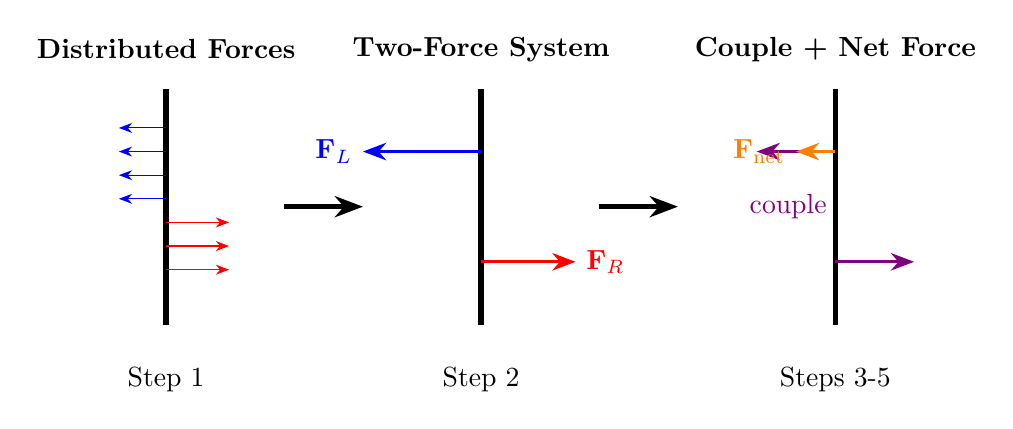
\begin{tikzpicture}[>=Stealth,scale=1.0]
    % Step 1-2: Distributed to two-force system
    \begin{scope}
        \node[align=center] at (0,3.5) {\textbf{Distributed Forces}};
        \draw[line width=2pt] (0,0) -- (0,3);
        
        % Multiple small forces
        \foreach \y in {2.5,2.2,1.9,1.6} {
            \draw[->,blue] (0,\y) -- (-0.6,\y);
        }
        \foreach \y in {1.3,1.0,0.7} {
            \draw[->,red] (0,\y) -- (0.8,\y);
        }
        
        \node at (0,-0.7) {Step 1};
    \end{scope}
    
    \draw[->,ultra thick] (1.5,1.5) -- (2.5,1.5);
    
    % Two equivalent forces
    \begin{scope}[shift={(4,0)}]
        \node[align=center] at (0,3.5) {\textbf{Two-Force System}};
        \draw[line width=2pt] (0,0) -- (0,3);
        
        \draw[->,very thick,blue] (0,2.2) -- (-1.5,2.2) node[left] {$\bvec{F}_L$};
        \draw[->,very thick,red] (0,0.8) -- (1.2,0.8) node[right] {$\bvec{F}_R$};
        
        \node at (0,-0.7) {Step 2};
    \end{scope}
    
    \draw[->,ultra thick] (5.5,1.5) -- (6.5,1.5);
    
    % Decomposed into couple + net force
    \begin{scope}[shift={(8.5,0)}]
        \node[align=center] at (0,3.5) {\textbf{Couple + Net Force}};
        \draw[line width=2pt] (0,0) -- (0,3);
        
        % Couple
        \draw[->,very thick,violet] (0,2.2) -- (-1.0,2.2);
        \draw[->,very thick,violet] (0,0.8) -- (1.0,0.8);
        \node[violet] at (-0.6,1.5) {couple};
        
        % Net force (leftover)
        \draw[->,very thick,orange] (0,2.2) -- (-0.5,2.2) node[left] {$\bvec{F}_{\text{net}}$};
        
        \node at (0,-0.7) {Steps 3-5};
    \end{scope}
\end{tikzpicture}
\caption{Forward dynamics decomposition: distributed forces (left) reduce to two equivalent forces on each side of the shaft (middle), which further decompose into a pure couple and a net force at the site of the dominant force (right).}
\label{fig:forward_decomposition}
\end{figure}

\subsection{Reverse Application to Inverse Dynamics}

In practice, we cannot directly apply this forward decomposition because inverse dynamics does not tell us where forces are applied or how they are distributed between hands. However, we can:

\begin{enumerate}
    \item \textbf{Set bounds on uncertainty:} Calculate the range of equivalent couples from the top to bottom of the grip (Equation~\ref{eq:couple_transform}). This range represents the maximum ambiguity in interpretation.
    
    \item \textbf{Conduct "what if" analyses:} Assume different force application patterns and calculate the resulting equivalent couples at those specific points. Compare these to assess sensitivity.
    
    \item \textbf{Integrate biomechanical constraints:} Use anatomical and motor control knowledge to rule out implausible force distributions, narrowing the space of viable interpretations.
\end{enumerate}

\section{Implications and Conclusions}

\subsection{The Fundamental Limitation}

Inverse dynamics provides dynamically equivalent representations, not unique physical descriptions. The method answers the question: ``What force-couple pair at this reference point would produce the observed motion?'' It does \emph{not} answer: ``What forces did the golfer actually apply, and where?''

This distinction is subtle but crucial. The equivalent couple at the midpoint is a mathematical convenience that depends on the choice of reference point. It may or may not correspond to actual twisting actions by the golfer.

\subsection{Practical Implications}

\textbf{For golf instruction:} Coaches should be cautious about interpreting inverse dynamics couples as direct indicators of what the golfer should ``feel'' or ``do.'' A large couple at the midpoint might arise from asymmetric force application rather than twisting.

\textbf{For biomechanics research:} Studies comparing golfers based on inverse dynamics torques should acknowledge that differences might reflect variations in \emph{where} forces are applied as much as \emph{how much} torque is generated. The alpha torque debate may be partially confounded by this ambiguity.

\textbf{For motor control theory:} The distributed nature of force application in golf (and other closed-loop tasks) suggests that the nervous system may not explicitly control "force" and "torque" as separate quantities. Instead, it may control forces at specific anatomical sites, which happen to produce particular force-couple combinations when reduced to a reference point.

\subsection{Future Directions}

To overcome the limitations identified here, future research could:

\begin{itemize}
    \item \textbf{Instrument the grip:} Pressure sensors or force plates embedded in the grip could directly measure force distributions, eliminating the need to infer them from inverse dynamics.
    
    \item \textbf{Combine inverse dynamics with optimization:} Use inverse dynamics for the golf club and inverse optimization for the golfer's hands/arms to find the most biomechanically plausible force distribution consistent with observed motion.
    
    \item \textbf{Develop sensitivity analyses:} Systematically explore how inverse dynamics interpretations change across the range of plausible force application patterns for each phase of the swing.
\end{itemize}

\subsection{Final Remarks}

The mathematical framework presented here does not invalidate inverse dynamics as a tool—it remains invaluable for understanding the mechanical demands of the golf swing. However, it does require that we interpret results with appropriate humility about what inverse dynamics can and cannot tell us.

When we see a force and couple in inverse dynamics output, we should ask: ``What range of physical force applications could produce this result?'' and ``Which of these is most biomechanically plausible given what we know about human motor control?'' 

By recognizing that the equivalent couple depends critically on where forces are applied—not just on what motions are produced—we can develop more nuanced and accurate understandings of skilled movement in golf and other closed-loop biomechanical systems.

\section*{Acknowledgments}

This work builds on discussions within the golf biomechanics community, particularly regarding the interpretation of inverse dynamics results and the ongoing debate about torque application patterns.

\end{document}
